\chapter{Compared results}

In this chapter we will compared the different data set to understand which parameters play an important role in the plasma formation, and identify the elements that are most efficient as clusters and dopant.
In the fist section we will show the average energy distribution of the electron VMI in order to compared to the recent data in the literature, additionally, we will present the different energy distribution for all the data sets to demonstrate the similarity to the spherical cloud model and the strong dependence between the Max energy and the Number of electron detected.
Second, we will compare the signal rates and mean values for droplets at different sizes, under NIR and MIR laser for He and Ne. Similarly, we will show the behaviour under different MIR pulse length for the two cluster elements. An intensity scan is also shown between NIR and MIR fields.  Finally we present the signal rates and mean values for the doping samples, first, just with Xe and second, with the different element, finishing presenting the result at Xe + Ca mix, where we found the most efficient system under MIR laser. 

\section{Energy distribution}

We compare the energy distribution of doped He clusters at different nozzle temperatures under two different laser pulses, a NIR laser of 800 nm with a pulse duration of 23 fs and Mid of 3200 nm and 45 fs pulse length.
The MID data was taken at 4 different nozzle temperatures with 30 mbr backing preassure and were doped with Xenon at a pressure of $0.0060$ mbar measured in the gas doping cell. The voltages were set to VMIx1  and the MCP and PHS to $1600$ V and $4000$ V respectively. The camera was set to minimum exposure time and the trigger system was used. 100000 pictures were taken for 4 different temperatures, at 10.6 K, 11 K, 12 K and 12.5 K. The data where evaluated once more as last section, demonstrating that the Trigger system worked efficiently. As result, it was shown that even for this high repetition laser rate, single shot signals can be achieved. The TOF signal work as a reference to identify the single explosion, and then each individual VMI picture is treated as follows. Fig \ref{fig:tofhe} shows a mean TOF for the measurement at 10.6 K. As we can see, there is a large amount of water and a small peak for hydrogen still in the vacuum chamber, this remain gases affect especially for the background. It is shown that Helium is effectively ionized due the peak at He$^{+}$ but on contrast no He$^{2+}$ signal was identify.

\begin{figure}[hbtp]
\centering
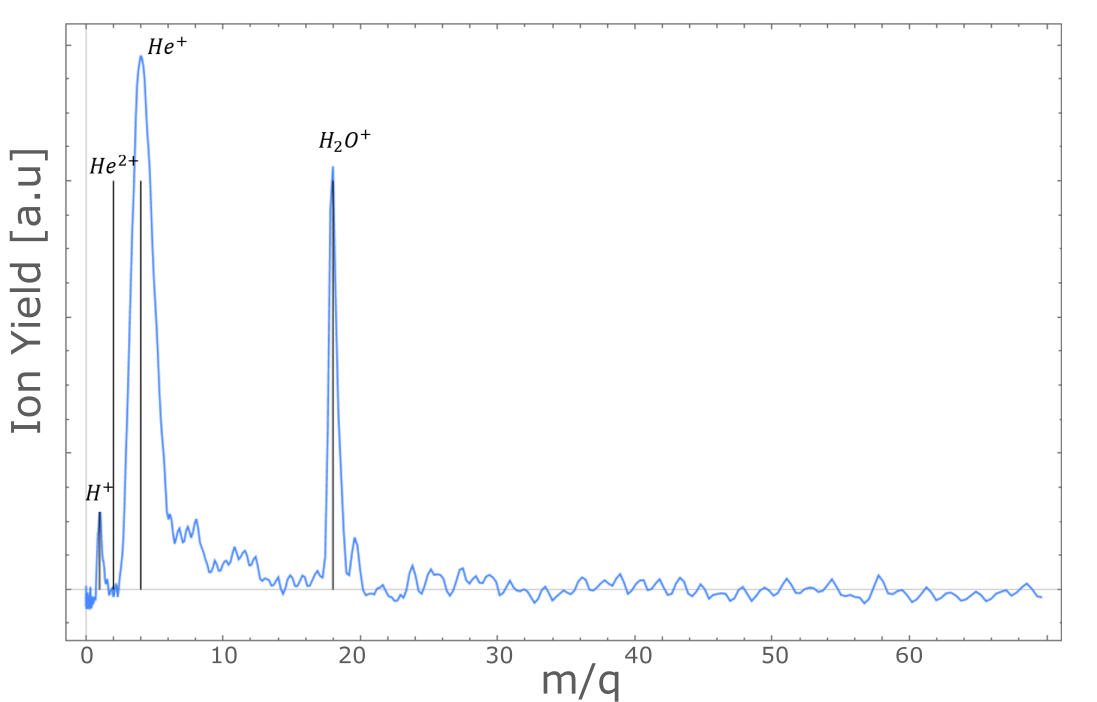
\includegraphics[width=0.7\textwidth]{../Images/TOF-10k6.png}
\caption[MIR TOF spectra He ]{Mean TOF spectra for He at 10.6 K}
\label{fig:tofhe}
\end{figure}

The cluster under NIR used 50 mbar backing preassure at 5 different nozzle temperatures, were doped with Xenon, with a doping pressure $0.0061$ mbar. The VMI were set to VMIx1 voltages and the MCP and PHS to 1250 V and 3400 V respectively. The camera was set to $\tau_{exp}=1$ ms exposure time. 50000 pictures were taken for 5 different temperatures, at 12.5 K, 13 K, 14 K, 16 K and 20 K. Using the Hagena scale \cite{hagena_cluster_1972}, we can calculate a prediction of the total number of atoms before and after the doping. Table \ref{tab:NIRclustersize} shows the  mean number of atom per cluster to at the different nozzle temperatures and also its corresponding number of dopant. 
\begin{figure}[hbtp]
\centering
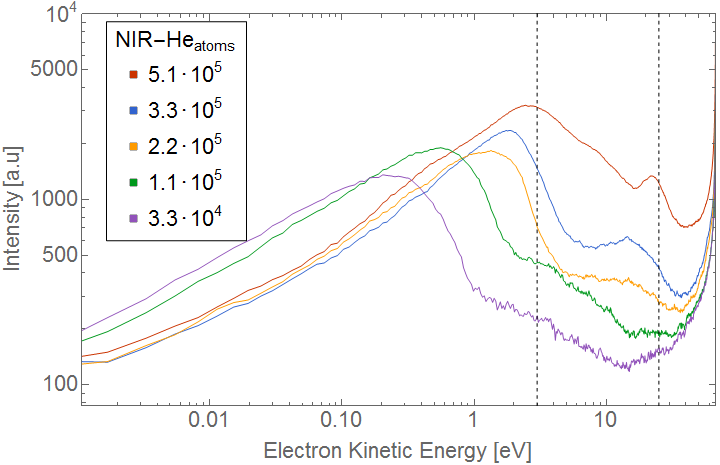
\includegraphics[width=0.9\textwidth]{../Images/results/Comparison_energyDistribution/NIR_He_summed_energydist.png} \\
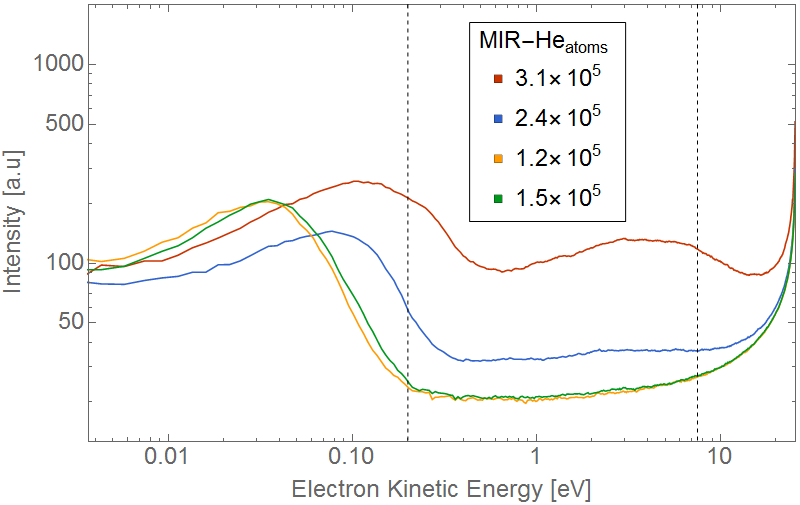
\includegraphics[width=0.9\textwidth]{../Images/results/Comparison_energyDistribution/MIR_He_summed_energydist.png} \\
\caption{Energy distribution for the summed individual coulomb explosion in He under NIR and MIR laser pulses at different temperatures}
\label{fig:MIR-NIrEnergssummed}
\end{figure}

We will compare the He energy distribution with the work of \textit{Kelberg et al}\cite{kelbg_auger_2019} where in Fig. 4 they present the energy dependence for three selected nozzle temperature with the mean droplet size  tuned to N$_{He}$ = 3.3E3, 3.6E4, and 2.2E6 atoms, under a constant NIR laser (810 nm) with an intensity of 4.5$\cdot$ 10$^{14}$ W$/$cm$^{2}$. To obtain a comparable mean energy, an inverse Abel transform on the summed images was perform in Pbasex  at 4 different temperatures in the MIR and 5 temperatures in the NIR.

Fig \ref{fig:MIR-NIrEnergssummed} top, show the calibrated electron kinetic energy distribution for the He droplets under the NIR laser with a laser intensity around 4E14 W$/$cm$^{2}$.  As shown, there exist a strong dependence on the droplet size and the signal intensity. The NIR data was taken with a MCP-PHs smaller, and this avoid to record higher energies, hence the data is accurate until 4 eV and we will not take into account the final tail of the plots in the right of the figure. Fortunately we can see that our energy distribution are quite similar to the ones in the literature, presenting continues behaviour in the lower energies, with a shoulder close to 0.1 ev and a second shoulder  close to 1 eV, as shown, thanks to our setup and the parameter used, we could achieve a better resolution for the low energies.

Fig \ref{fig:MIR-NIrEnergssummed}  bottom, was proceeded in the same way as above, showing an energy distribution up to 25 eV. As shown, both graph have a similar distribution in their corresponding energies, where the values close to 0 has the highest electron density while the lower energies tends to be at lower intensity.more over, the MIR data also present the first shoulder around 0.1 eV but the second shoulder is exhibit close to 5eV. This features can also be identified in Kelberg´s work, where the shoulders are present for the biggest droplets on 1 and 6 eV respectively, close to the values we do.

\section{Cluster Size Dependence}

This section compares the cluster size of He and Ne under MIR and NIR laser pulses. The He clusters under MIR and NIR used the same parameters above respectively, while the Ne cluster were just used under the MIR laser and were created at 5 nozzle temperature 39, 40, 41, 42 and 44 K with a backing pressure of $P_{0}=50$ mbar. Xenon where introduce at a fix  pressures measured in the doping cell of 0.00036 mbar. The VMI voltages  were set to VMIx1  and the MCP and PHS to $1800$ V and $4100$ V respectively. The camera was stablish to exposure time of $t_{exp}=34$ $\mu$s   with the single shoot measurement scheme. The laser power were set to an average power of 11 W ($\sim$ 2E14 W/cm$^{2}$).

\begin{figure}[h!]
\begin{subfigure}[l]{0.32\textwidth}
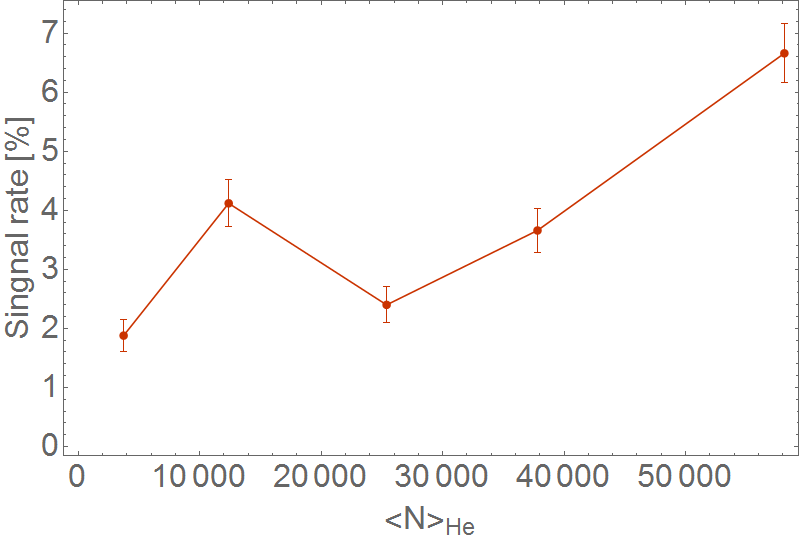
\includegraphics[width=1\textwidth]{../Images/results/NI_He_Dropletsize/signalrate.png} \caption{NIR-He Signal rate} \end{subfigure}
\begin{subfigure}[l]{0.32\textwidth}
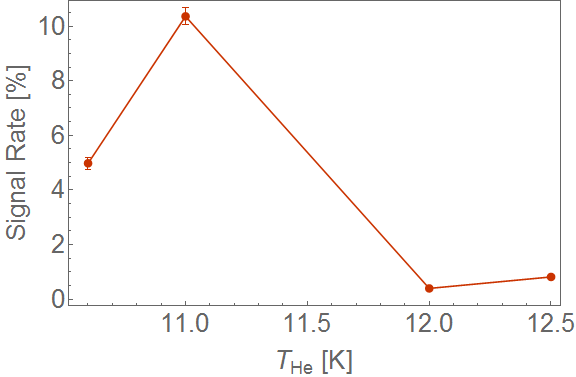
\includegraphics[width=1\textwidth]{../Images/results/Mir_He_Dropletsize/sigrate.png}
\caption{MIR-He Signal rate} \end{subfigure}
\begin{subfigure}[l]{0.32\textwidth}
\includegraphics[width=1\textwidth]{../Images/results/MIR_Ne_DropletSize/Sigrate.png}
\caption{MIR-Ne Signal rate} \end{subfigure}
\caption[Cluster size-signal rate]{Signal rate cluster size dependence for He cluster under NIR and MIR laser and Ne cluster under MIR.}
\label{fig:CompSigRate}
\end{figure}

Fig \ref{fig:CompSigRate} shows the signal rate for the different nozzle temperature and cluster element. As shown is easy to evaluate that the droplet size acts directly proportional to the signal rate, in other words. the bigger droplets  are more easy to ignite. As we can see in a and c, the higher nozzle temperature contains the lower rates while the lower temperatures contains rates up to 12$\%$. On b, the cluster size at 10.5 K shows a reduction in the cluster size, In this case we need to analyze it independently, because at 11 K xxxxxxx.

\begin{figure}[h!]
\begin{subfigure}[l]{0.32\textwidth}
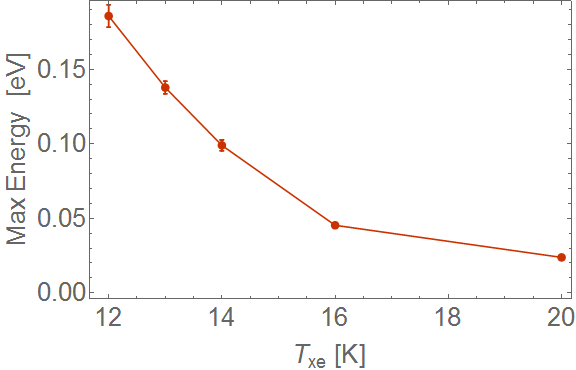
\includegraphics[width=1\textwidth]{../Images/results/NI_He_Dropletsize/MeanElec.png} 
%\caption{NIR-He Mean Num e-}
\end{subfigure}
\begin{subfigure}[l]{0.32\textwidth}
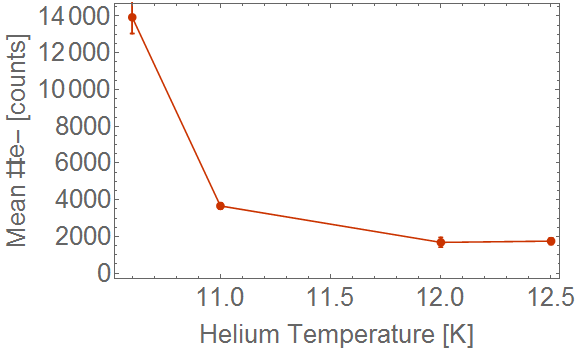
\includegraphics[width=1\textwidth]{../Images/results/Mir_He_Dropletsize/Meanelec.png} 
%\caption{MIR-He Mean Num e-}
\end{subfigure}
\begin{subfigure}[l]{0.32\textwidth}
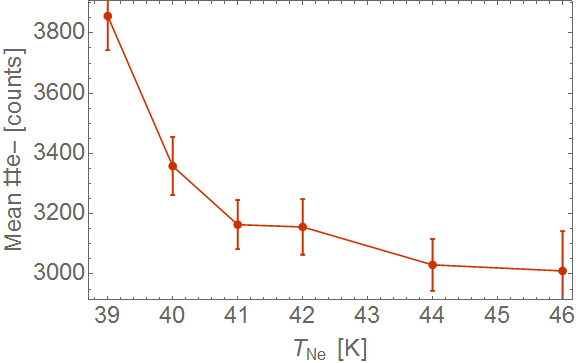
\includegraphics[width=1\textwidth]{../Images/results/MIR_Ne_DropletSize/MeanElec.png} 
%\caption{MIR-Ne Mean Num e- }
\end{subfigure}

\begin{subfigure}[l]{0.32\textwidth}
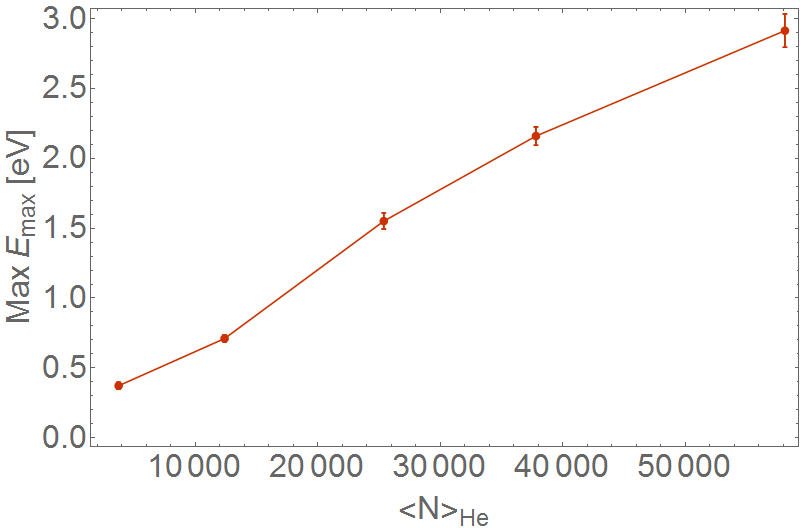
\includegraphics[width=1\textwidth]{../Images/results/NI_He_Dropletsize/MeanEnerg.png} 
\caption{NIR-Helium }\end{subfigure}
\begin{subfigure}[l]{0.32\textwidth}
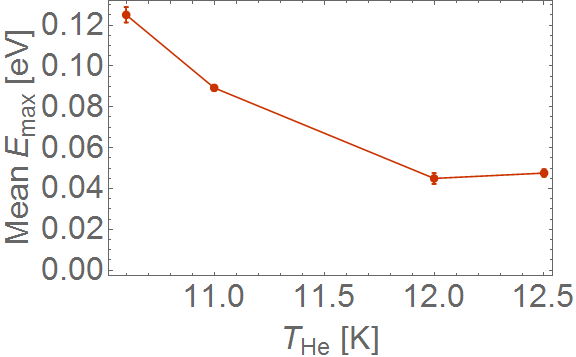
\includegraphics[width=1\textwidth]{../Images/results/Mir_He_Dropletsize/MeanEnerg.png} 
\caption{MIR-Helium }\end{subfigure}
\begin{subfigure}[l]{0.32\textwidth}
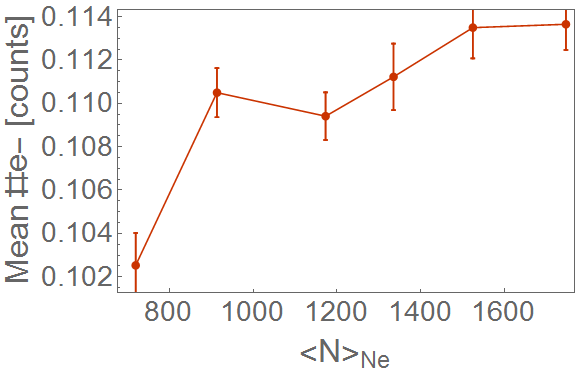
\includegraphics[width=1\textwidth]{../Images/results/MIR_Ne_DropletSize/MeanEnerg.png} 
\caption{MIR-Neon  }\end{subfigure}
\caption[Cluster size- Mean values]{Mean values for cluster size dependence for He  under NIR and MIR laser and Ne cluster under MIR.}
\label{fig:ClusterSizemean}
\end{figure}

Once the signal is identified as a single explosion, the central bloop is analysed convert it to maximal Kinetic energy and Number of electrons. Fig \ref{fig:ClusterSizemean} shows the mean values for each data set, on top, the mean values for the number of electrons in counts, and on bottom, the mean value for the Max energy in eV. As we can see, both sets present a similar tendency where the higher temperature has either low brightness and low energy. As explained in chapter 3, we assume the coulomb explosion as a uniformly electronic cloud, in this case, two affirmations can be done. First, The mean value of the He clusters in NIR compared to the MIR is almost two order of magnitude higher, this suggests that the NIR electronic cloud is denser because the energies remains comparable, similarly  the two experiment under MIR has values in the same order of magnitude suggesting that the NIR is more efficient in the plasma production that the MIR. Second, we confirm our presumption that in the signal rate the bigger droplets are easy to ignite. As shown, the lower temperatures contains the highest signal rates, and in the same way the highest mean values. This behaviour is expected because the bigger the droplet, more electrons are available in the system, so more electron will be detected. If we assume a comparable density, we also expect that the mean energies rises as the data confirms. Furthermore, the Ne mean values shows a similar behaviour but less acute, although the values keeps relatively constant and don't change as fast as the He clusters, it does show a reduction in the same direction, specially the mean number of electrons denote a strong correlation with the signal rate and we can expect that  this tendency remains independent the cluster element.

In brief, t´he efficiency for the plasma  formation increase with the cluster size, independing of the cluster element. This could be explain if we compare the potential of each size, clearly, the bigger droplet have deeper potential where the ionized electron will be trap, hence they will be trap and interact with the laser field. in contrast, for the smaller droplets, th potential can be not strong enougth to cath the electrons, escaping from the cluster with out starting the ignition process. 

\section{Pulse Scan Dependence}

One of the advantage of the laser system in ELI-Alps, is the possibility to change the laser pulse duration, in this section  we compares the pulse duration of MIR laser on He and Ne cluster. 

Helium clusters at the same nozzle temperature $T_{nozzle}=10.5$ K and  backing pressure of $P_{0}=30$ mbar, were doped with Xenon at a fix doping level $P_{dop}=2.4E-4$ mbar pressure measured in the gas doping cell. At this nozzle temperature the Helium forms big clusters, with approximated $N=3150000$ atoms before going through the oven chamber and its doped with Xe$_{dop}$=75 atoms. The VMI voltages were set to VMIx1 and the MCP and PHS to $1600$V and $4000$V respectively. The camera was stablish to a exposure time of $t_{exp}=34 \mu$s. A first averaged mode signal was taken as a guide to the eye and after 100000 pictures were taken at 4 different pulse duration, at $65, 120, 200$ and $250$  fs, measured by the ELI-laser personal supporting us in the experiment, using FROG technique.
In the beginning of the experiment, we notice that the laser pulse have a dependence with the laser power, longer pulses results in a weaker power. Table \ref{tab:pulsepower} resume the laser power obtained for each of the pulse duration. Fortunately the intensities didn't defer much and the intensities obtained are farther that the threshold to start the coulomb explosion as seen in the intensity scan above.
  
   
\begin{table}[]
\centering
\label{tab:pulsepower}
\begin{tabular}{|l|l|c|}
\hline
Pulse duration {[}fs{]} & \multicolumn{1}{c|}{Power{[}mW{]}} & Laser intensity {[}W/cm$^{2}${]} \\ \hline
65 & 8.8 & 1.5E14 \\ \hline
120 & 9.7 & 8E13 \\ \hline
200 & 9.8 & 5E13 \\ \hline
250 & 9.2 & 3.9E13 \\ \hline
\end{tabular}
\caption{MIR laser power-pulse duration dependence for He clusters}
\end{table}

Neon cluster used a fix doping level with Xenon at a nozzle temperature 39 K and a backing pressure of $P_{0}=50$ mbar were shoot by the MIR laser pulse at 5 different pulse duration of, 48, 55, 64 71, and 94 fs. Xenon were introduce at a fix pressures measured in the doping cell at 0.0002 mbar. The VMI voltages were set to VMIx1 and the MCP and PHS to $1700$ V and $4000$ V respectively. The camera was stablish to exposure time of 34 $\mu$s with the single shoot measurement scheme. As above the pulse duration have a recurrent effect in the laser power. Unfortunately, at the end of the beam time the laser technicians realized that a BMO crystal was still in the beam pad during the hole experiment, so we needed to rescale our pulse duration and in consequence no data with pulses further than 105 fs was taken. Table \ref{tab:Neonpulsepower} shows the different powers and consecutive the laser intensities at each data set was taken, as shown all sets are comparable.

\begin{table}[t]
\centering

\begin{tabular}{|l|l|c|}
\hline
Pulse duration {[}fs{]} & \multicolumn{1}{c|}{Power{[}W{]}} & Laser intensity {[}W/Cm$^{2}${]} \\ \hline
48 & 10.5 & 2E14 \\ \hline
55 & 11 & 1.7E14 \\ \hline
64 & 11 & 1.5E14 \\ \hline
71 & 10.4 & 1.3E14 \\ \hline
94 & 8.6 & 1E14 \\ \hline
\end{tabular}
\caption{Neon pulse scan  intensity table.}
\label{tab:Neonpulsepower}
\end{table}

\begin{figure}[h!]
\begin{subfigure}[l]{0.48\textwidth}
\caption{MIR-Helium}
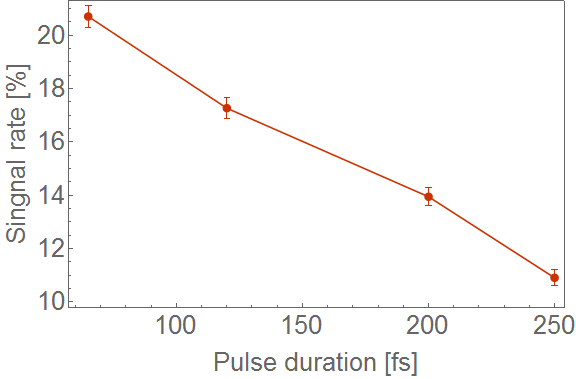
\includegraphics[width=1\textwidth]{../Images/results/MIR_He_pulsescan/raw/signalrate.png} %
\end{subfigure}
\begin{subfigure}[l]{0.48\textwidth}
\caption{MIR-Neon}
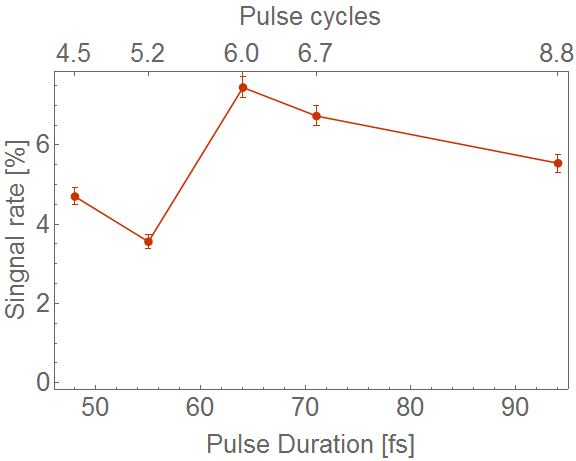
\includegraphics[width=1\textwidth]{../Images/results/MIR_Ne_pulseduration/SigRate.png} %\caption{MIR-
\end{subfigure}


\begin{subfigure}[l]{0.48\textwidth}
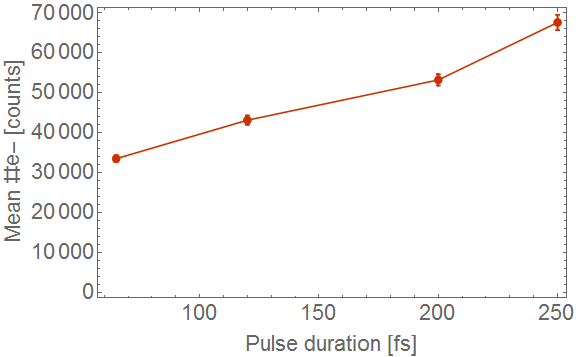
\includegraphics[width=1\textwidth]{../Images/results/MIR_He_pulsescan/raw/meanelect.png} 
\end{subfigure}
\begin{subfigure}[l]{0.48\textwidth}
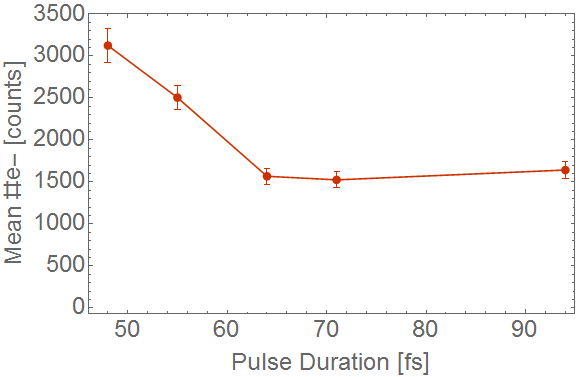
\includegraphics[width=1\textwidth]{../Images/results/MIR_Ne_pulseduration/MeanElec.png} 
\end{subfigure}

\begin{subfigure}[l]{0.48\textwidth}
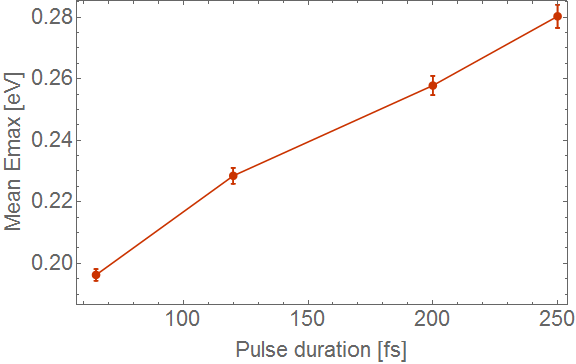
\includegraphics[width=1\textwidth]{../Images/results/MIR_He_pulsescan/raw/meanenergt.png} 
\end{subfigure}
\begin{subfigure}[l]{0.48\textwidth}
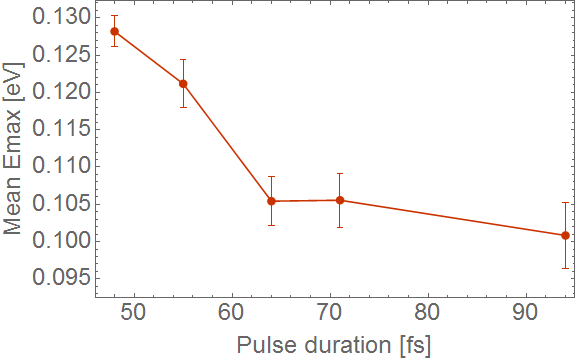
\includegraphics[width=1\textwidth]{../Images/results/MIR_Ne_pulseduration/MeanEnerg.png} 
\end{subfigure}

\caption[Cluster size- Mean values]{Mean values for cluster size dependence for He  under NIR and MIR laser and Ne cluster under MIR.}
\label{fig:pulsemean}
\end{figure}

Fig \ref{fig:pulsemean} shows the signal rate and mean values for the He cluster and Ne clusters pulse  duration dependence. On top, the signal rates for He shows an expected relation where the longer the pulse the lower the signal rate linearly. This behaviour is expected because as  explained, the longer pulse duration the lower the intensity of the beam, in consequence, there will be less energy available to ignite the plasma. The Ne signal rate on contrary shows a more constant relation, oscillating around 4 to 6$\%$. It is difficult to find a pattern because of the first two points are alter respect to the other three, but in general we can suppose it keeps constant behaviour.

On the mean values of fig \ref{fig:pulsemean} we appreciate a non trivial relation in the He clusters.     Even though the signal rate is decreasing with the pulse length, the mean values of energy and number of electrons increase. Although, it is a non-intuitive results, it can be explained if we take into account the number of cycles in the pulse, longer pulses gives more cycles to the electrons to interact with. In consequence, yet the initial ionization probability is lower, the electrons created on the first cycles of the pulse will have more time to interact with the laser field, acquiring more energy and incrementing the electronic cascade that will start the coulomb explosion. The Energy mean values confirm this assumption as the longer pulses give higher energies.
On contrary, we can not identify this effect on the Ne clusters. It can be due the lack of data at long cycles or it can means the cluster element does play a role. As shown, the mean Num electron remain constant for the last three points while the fist goes up to 3000 e-. It important to notice the two first point in the He measn values are at short pulses, not covered by the He plot, what makes eit difficul to compare them directly, nevertheless the other three points are. If we examine carefully, for  pulses length bewtween 60 and 100 fs the signal rate in He and Ne shows a similar behaoviour, same for the Mean num of electrons, Althoug the changes are samll, we can specte that this dynamic continues for longer tiems. further, the mean energy present little change aswell. Considering the number of cycles between the plot we see that the data taken in He present number 4 time bigger in the number of cycles, while the comparable points in Ne are just from 6 to 9 cycles. 


\section{Intensity scan}

In this data set we compare the signal rate of the He clusters Under NIR and MIR atz different laser intensities. The laser system used At the Max plank institute at Heidelberg was a NIR laser at $800nm$ wavelength and a rate of $10Hrz$ and a $d_{pulse}=23$ fs pulse duration. Helium clusters at the same nozzle temperature $T_{nozzle}=12.2$ K and  backing pressure of $P_{0}=45$ mbar, were doped with Xenon at a fix doping level, with the a constant pressure measured in the oven chamber of $P_{oven}=2E-6$ mbar. This measurement where taken with a slightly smaller MCP-PHS arrangement of $d=42.2mm$ diameter of active area. At this nozzle temperature the Helium droplet have proximate $N=397390$ atoms before going through the oven chamber and its doped with $Xe_{dop}=134$ atoms, given a final number of He number of $N=386596$ atoms. The VMI voltages where set to VMIx2 and the MCP and PHS to $1250$ V and $4000$ V respectively. The camera was stablish to exposure time of $t_{exp}=1$ ms. 50000 pictures were taken for 7 different laser power, at $55,80,115,140,185,210$ and $240$ mW. 

\begin{figure}[h!]
\begin{subfigure}[l]{0.48\textwidth} \caption{NIR-Helium}
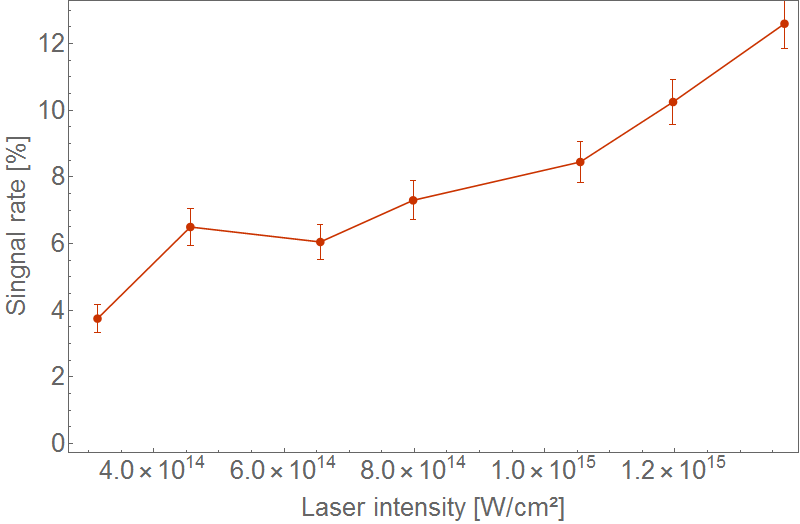
\includegraphics[width=1\textwidth]{../Images/results/NIR_He_intensityscan/signalrate.png} \end{subfigure}
\begin{subfigure}[l]{0.48\textwidth} \caption{MIR-He Signal rate} 
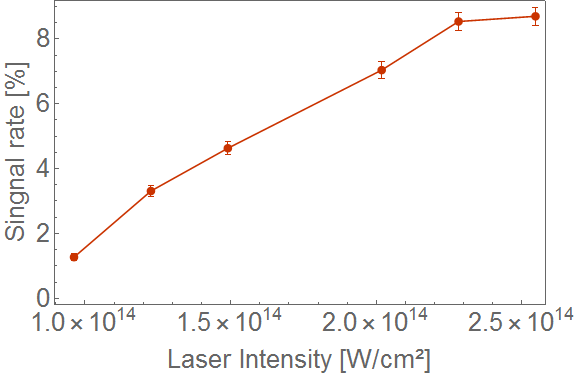
\includegraphics[width=1\textwidth]{../Images/results/MIR_He_waterIntensityscan/sigRate.png}\end{subfigure}
\caption[Intensity scan-signal rate]{Signal rate for He and Ne clusters under a NIR and MIR laser at different intensities.}
\label{fig:IntensitySigRate}
\end{figure}

Additionally, the laser system used at ELI-Alps was at $3200$ nm wavelength and a rate of $100$ KHz and a $\tau_{pulse}=45$ ps pulse duration. Helium clusters at the same nozzle temperature $T_{nozzle}=11$ K and  backing pressure of $P_{0}=30$ mbar, were doped with Water at a fix doping level $P_{dop}=1E-4$ mbar pressure measured in the gas doping cell. At this nozzle temperature the Helium droplet have proximate $N=215972$ atoms before going trough the oven chamber and its doped with H$_{2}$O$_{dop}$=56 atoms. The VMI voltages were set to VMIx1 and the MCP and PHS to $1750$V and $4000$V respectively. The camera was stablish to exposure time of $t_{exp}=34 \mu$s. 100000 pictures were taken for 6 different laser power, at $2, 4, 6, 7, 8$ and $9.5$ W, measured before the laser beam enters to the detection chamber and its back focus by the mirror. 

Fig \ref{fig:IntensitySigRate} shows the signal rate for the different lasers. As shown, the rates independent of the wavelength increase with the intensities, so two assumptions can be done. First, the laser intensity play a fundamental role in given the starting condition to the nanoplasma, it behaves directly proportional to the plasma production efficiency. Additionally, we can assume that for intensities lower than 1E14 W/cm$^{2}$ the rate tends to zero. this behaviour is expected because as explained, laser power is not enough to Ionized He by itself, so the Initial dopant ionization is needed to start the process, if the intensity is not sufficient there will be no electrons to interact with the laser pulse and nothing will happen. 

\section{Xenon Doping Scan}

For this section we will compare the plasma formation on Ne and He cluster under the MIR laser doped with Xenon at different levels. The Helium clusters were created at the same nozzle temperature $T_{nozzle}=10.6$ K and a backing pressure of $P_{0}=30$ mbar. Xenon were introduce at 5 different pressures measured in the gas doping cell. The VMI voltages were set to VMIx1 and the MCP and PHS to $1600$V and $4000$V respectively. The camera was stablish to exposure time of $t_{exp}=34 \mu$s and single shot was ensure. The laser power was monitored constantly guarantee an average power of 10.7 W at pulses duration around $45$ fs.

Neon clusters were created at $T_{nozzle}=39$ K and at a backing pressure of $P_{0}=50$ mbar. Xenon was introduce at 7 different pressures measured in the oven chamber. The VMI voltages were set to VMIx1 and the MCP and PHS to $1700$ V and $4000$ V respectively. The camera was stablish to an exposure time of $t_{exp}=34$ $\mu$s  and the laser power was set to an average of 10 W.


\begin{figure}[h!]
\begin{subfigure}[l]{0.48\textwidth} \caption{MIR-Helium}
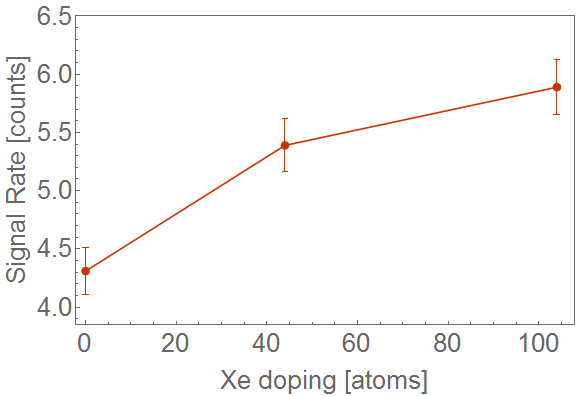
\includegraphics[width=1\textwidth]{../Images/results/MIR_He_XeCaDop/Xe_SignalRate.png}  \end{subfigure}
\begin{subfigure}[l]{0.48\textwidth} \caption{MIR-Neon } 
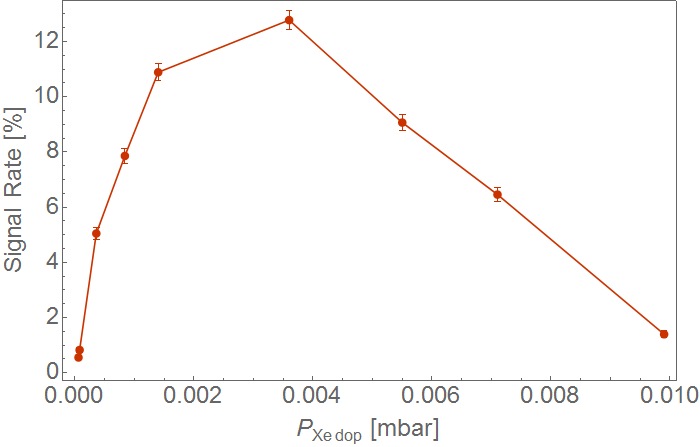
\includegraphics[width=1\textwidth]{../Images/results/MIR_Ne_XeDop_39K/SigRate.png} \end{subfigure}
\caption[Xe doping scan-signal rate]{  Signal rate for He and Ne clusters under a NIR and MIR laser at different Xe doping levels.}
\label{fig:IntensitySigRate}
\end{figure}

\begin{figure}[h!]
\begin{subfigure}[l]{0.48\textwidth} \caption{MIR-Helium}
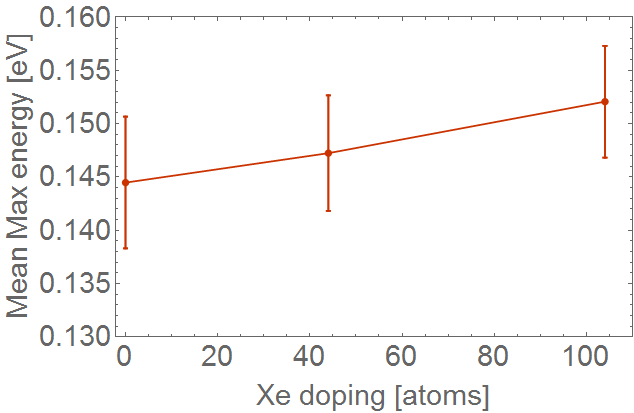
\includegraphics[width=1\textwidth]{../Images/results/MIR_He_XeCaDop/Xe_Meanenerg.png}  \end{subfigure}
\begin{subfigure}[l]{0.48\textwidth} \caption{MIR-Neon } 
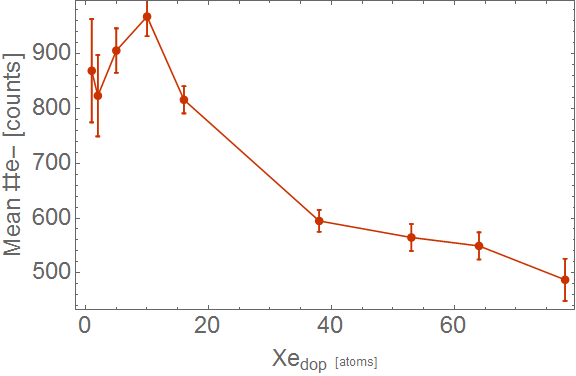
\includegraphics[width=1\textwidth]{../Images/results/MIR_Ne_XeDop_39K/MeanEnerg.png} \end{subfigure}

\begin{subfigure}[l]{0.48\textwidth} 
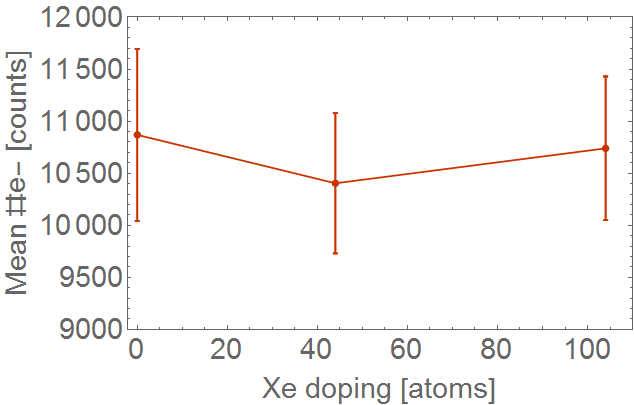
\includegraphics[width=1\textwidth]{../Images/results/MIR_He_XeCaDop/Xe_Meanelec.png}  \end{subfigure}
\begin{subfigure}[l]{0.48\textwidth}
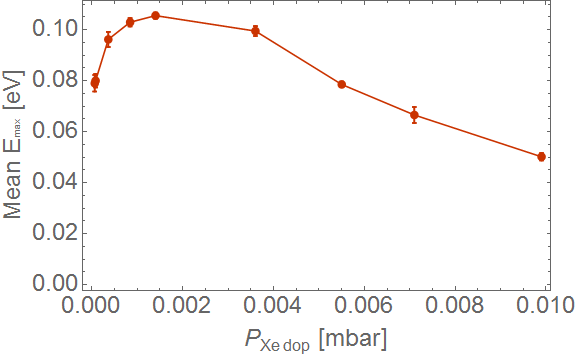
\includegraphics[width=1\textwidth]{../Images/results/MIR_Ne_XeDop_39K/MeanElec.png} \end{subfigure}
\caption[Xe doping scan-signal rate]{Signal rate for He and Ne clusters under a NIR and MIR laser at different Xe doping levels.}
\label{fig:IntensitySigRate}
\end{figure}

